\item[(d)]
\section*{Task (d)}

\subsection*{Problem Statement}
Perform the same steps as in (c), but without multiplying the signal blocks by a Hamming window. How does the resulting magnitude diagram of the STFT differ from the one computed in (c)? How is the effect called that causes this difference?

\subsection*{Python Script}
\begin{verbatim}
import numpy as np
import matplotlib.pyplot as plt
from scipy.io import wavfile
import os

# Create fig directory if it doesn't exist
if not os.path.exists('fig'):
    os.makedirs('fig')

# Read the DTMF signal from the WAV file
fs, signal = wavfile.read('dtmf.wav')

# Parameters for STFT
block_length = 256  # Block length
overlap = block_length // 2  # Overlapping factor of 2

# Pad the signal with zeros if necessary
padding_length = (block_length - len(signal) % block_length) % block_length
padded_signal = np.append(signal, np.zeros(padding_length))

# Generate signal blocks
num_blocks = (len(padded_signal) - overlap) // (block_length - overlap)
blocks = np.zeros((num_blocks, block_length))

for i in range(num_blocks):
    start = i * (block_length - overlap)
    end = start + block_length
    blocks[i, :] = padded_signal[start:end]

# Compute the FFT for each block
ftbs = np.fft.fft(blocks, axis=1)

# Generate the time and frequency vectors for plotting
f_stft = np.fft.fftfreq(block_length, 1/fs)[:block_length // 2]
t_stft = np.arange(num_blocks) * (block_length - overlap) / fs

# Plot the STFT magnitude without Hamming window
plt.figure(figsize=(12, 6))
plt.pcolormesh(t_stft, f_stft, np.abs(ftbs[:, :block_length // 2].T), shading='gouraud')
plt.title('STFT Magnitude of DTMF Signal Without Hamming Window')
plt.xlabel('Time (s)')
plt.ylabel('Frequency (Hz)')
plt.colorbar(label='Magnitude')
plt.ylim(0, 2000)  # Limit the frequency range to 0-2000 Hz
plt.savefig('fig/ex4_d_stft_magnitude_no_hamming.png')
plt.show()
\end{verbatim}

\subsection*{STFT Magnitude of the DTMF Signal Without Hamming Window}
\begin{figure}[h]
    \centering
    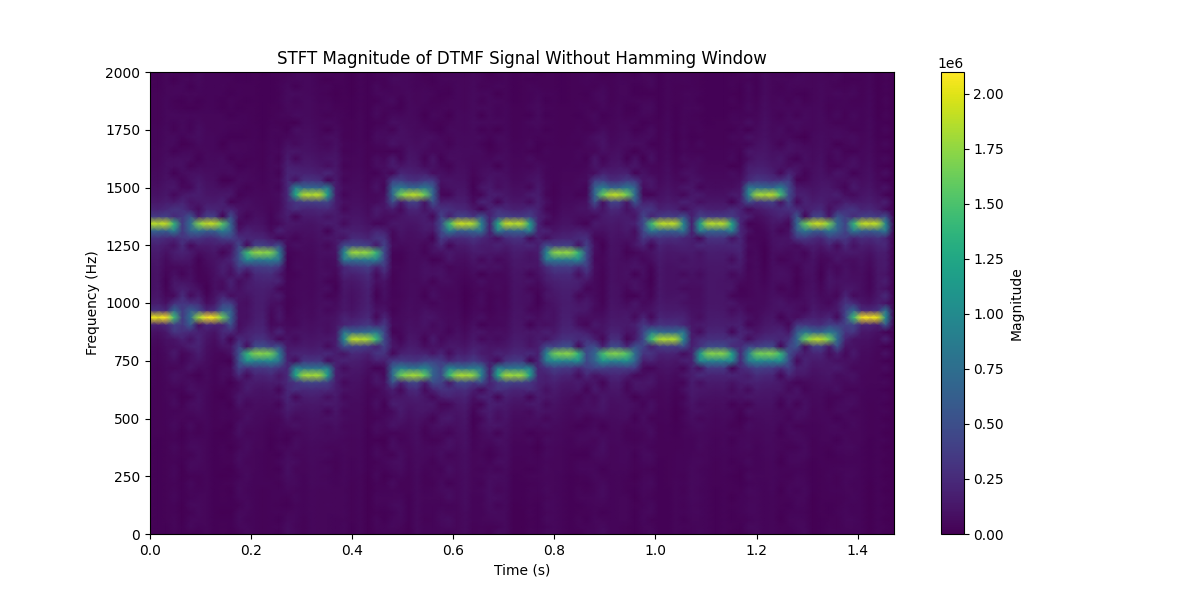
\includegraphics[width=0.8\textwidth]{fig/ex4_d_stft_magnitude_no_hamming.png}
    \caption{STFT Magnitude of the DTMF Signal Without Hamming Window}
    \label{fig:ex4_d_stft_magnitude_no_hamming}
\end{figure}

\subsection*{Analysis}
The resulting magnitude diagram of the STFT without the Hamming window shows more spectral leakage compared to the one computed with the Hamming window in Task (c). Spectral leakage occurs because the signal blocks are treated as if they are periodic, leading to discontinuities at the block edges. These discontinuities cause the energy to spread across multiple frequencies, resulting in a less clear representation of the signal's frequency content.
